% DASFAA paper template based on Springer's LLNCS macro package.
%
\documentclass[runningheads]{llncs}
%

\usepackage[T1]{fontenc}
%

\usepackage{graphicx}
% Used for displaying a sample figure. If possible, figure files should
% be included in EPS format.
%
% If you use the hyperref package, please uncomment the following two lines
% to display URLs in blue roman font according to Springer's eBook style:
\usepackage{color}
%\renewcommand\UrlFont{\color{blue}\rmfamily}
%\urlstyle{rm}

\usepackage[ruled, vlined, linesnumbered]{algorithm2e}
\usepackage{amsfonts, amsmath}
\usepackage{bm}
\usepackage{booktabs} 
%\usepackage[utf8]{inputenc}
\usepackage{pifont}
\usepackage{xcolor, xspace}
\usepackage{multirow}
\usepackage{cite}
\usepackage{placeins}
\usepackage{tikz}
\usetikzlibrary{arrows.meta,positioning}


%
\begin{document}
%
\title{Towards Federated LoRA Fine-tuning with Rank Heterogeneity}
%
%\titlerunning{Abbreviated paper title}
% If the paper title is too long for the running head, you can set
% an abbreviated paper title here
%
\author{Anonymous}
%
\authorrunning{Anonymous}
\institute{Anonymous}

% \author{First Author\inst{1}\orcidID{0000-1111-2222-3333} \and
% Second Author\inst{2,3}\orcidID{1111-2222-3333-4444} \and
% Third Author\inst{3}\orcidID{2222--3333-4444-5555}}
% %
% \authorrunning{F. Author et al.}
% % First names are abbreviated in the running head.
% % If there are more than two authors, 'et al.' is used.
% %
% \institute{Princeton University, Princeton NJ 08544, USA \and
% Springer Heidelberg, Tiergartenstr. 17, 69121 Heidelberg, Germany
% \email{lncs@springer.com}\\
% \url{http://www.springer.com/gp/computer-science/lncs} \and
% ABC Institute, Rupert-Karls-University Heidelberg, Heidelberg, Germany\\
% \email{\{abc,lncs\}@uni-heidelberg.de}}
%
\maketitle              % typeset the header of the contribution
%



\newcommand{\etal}{\textit{et~al.}\xspace}
\newcommand{\eg}{\textit{e.g.},\xspace}
\newcommand{\ie}{\textit{i.e.},\xspace}
\newcommand{\etc}{etc.\xspace}

\newcommand\figref[1]{Fig.~\ref{#1}}
\newcommand\algref[1]{Algorithm~\ref{#1}}
\newcommand\tabref[1]{Table~\ref{#1}}
\newcommand\secref[1]{Sec.~\ref{#1}}
\newcommand\equref[1]{Eq.~(\ref{#1})}
\newcommand\thmref[1]{Theorem ~\ref{#1}}
\newcommand\lemmaref[1]{Lemma ~\ref{#1}}
\newcommand\assumptionref[1]{Assumption ~\ref{#1}}
\newcommand\appref[1]{Appendix~\ref{#1}}
\newcommand\defref[1]{Definition~\ref{#1}}

\newcommand{\fakeparagraph}[1]{\vspace{1mm}\noindent\textbf{#1.}}
\newcommand{\sysname}{\text{DualAda}\xspace}

\newcommand{\algnote}[1]{\textcolor{blue}{\tt{// #1}}}

\ifodd 1
\newcommand{\TODO}[1]{\textbf{\color{red}{TODO: #1} }}
\newcommand{\TBD}[1]{\textbf{\color{blue}{TBD: #1} }}
\newcommand{\zimu}[1]{{\color{brown}{#1}}}
\newcommand{\boyi}[1]{{\color{blue}{#1}}}
\newcommand{\mym}[1]{{\color{teal}{#1}}}

% \newcommand{\todis}[1]{\textbf{{\color{teal}{TO DISCUSS: #1}}}}
% \else
% \newcommand{\TODO}[1]{#1}
% \newcommand{\zimu}[1]{#1}
% \newcommand{\boyi}[1]{#1}
% \newcommand{\mym}[1]{#1}
% \fi



\begin{abstract}


\end{abstract}


\section{Introduction}
\label{sec:intro}

Federated fine-tuning enables multiple clients to adapt a pretrained language
model collaboratively while keeping their private data decentralized.
Combined with parameter-efficient adaptation such as LoRA~\cite{hu2022lora},
federated fine-tuning avoids transmitting the full language model and has been
used to adapt large language models to decentralized instruction and task data
without collecting raw client examples~\cite{mcmahan2017fedavg,zhang2024fedit,sun2024ffalora}.

The standard approach gives every client a LoRA adapter with the same rank and
aggregates the corresponding factors across clients \cite{zhang2024fedit}.
However, clients in a federated deployment may have substantially different
memory, compute, and communication budgets \TODO{refs}.
Assigning the same LoRA rank to all clients either exceeds the resources of
constrained clients or leaves the capacity of stronger clients underused.
A natural way to accommodate this resource heterogeneity is to assign client
$i$ a fixed rank budget $r_i$ and let clients fine-tune adapters with different
ranks~\cite{bai2024flexlora,wang2024flora,cho2024hetlora}.
This change makes cross-client aggregation nontrivial: although the effective
updates $B_iA_i$ have the same output shape, the factor matrices have
rank-dependent inner dimensions and cannot be directly averaged.

Existing rank-heterogeneous methods resolve this incompatibility by introducing
additional server-side operations, but they incur important trade-offs, 
\eg high communication cost~\cite{wang2024flora} or lack of fairness guarantees across clients~\cite{bai2024flexlora}.
In this paper, we explore \textit{Selective Rank Sharing}, a simple and
communication-efficient approach to rank-heterogeneous federated LoRA
fine-tuning.
As shown in \figref{fig:selective-rank-sharing}, each client partitions its fixed rank budget into a globally shared prefix and a client-specific protected remainder.
Only the shared prefix is aggregated and broadcast, while both portions remain trainable locally.
This design preserves each client's total rank budget and avoids requiring
full-size adapter communication or server-side SVD for rank redistribution.

We further conduct motivation experiments on FLAN~\cite{wei2022finetuned} with eight clients, assigning fixed rank budgets of 16 and 64 to four clients each (see \figref{fig:acl-motivation}).
The experiments reveal two observations.
\textit{(i)} Changing the shared-prefix width affects rank groups differently: a
width that improves one group can hurt another, and the same width consumes
different fractions of clients' rank budgets.
\textit{(ii)} At a fixed shared width, the relative cosine similarity of same-rank and same-domain updates varies across the two rank groups and training rounds.
These geometric differences leave open how external updates affect each client's task performance.
These observations lead to the following two challenges.

\begin{figure}[!t]
    \centering
    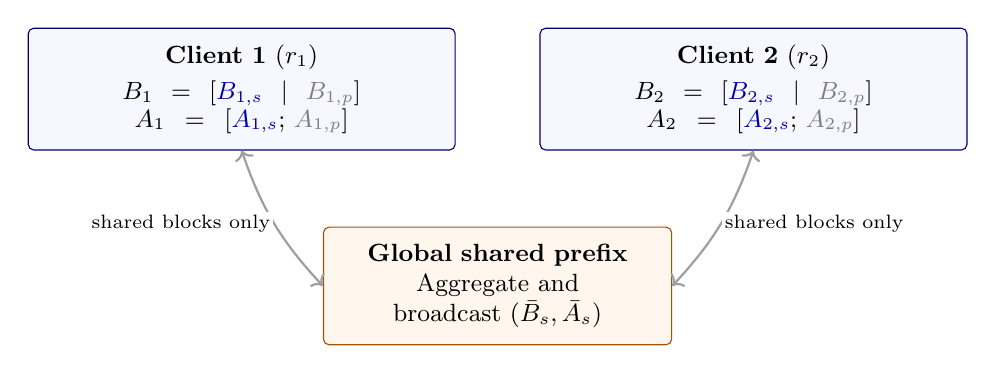
\begin{tikzpicture}[
        client/.style={draw=blue!45!black, fill=blue!3, rounded corners=2pt,
            text width=5.0cm, align=center, inner sep=6pt, font=\small},
        server/.style={draw=orange!65!black, fill=orange!7, rounded corners=2pt,
            text width=4.0cm, align=center, inner sep=6pt, font=\small},
        sync/.style={<->, thick, draw=gray!75}
    ]
        \node[client] (client1) at (-3.25,1.35) {\textbf{Client 1} ($r_1$)\\[2pt]
            $B_1=[\textcolor{blue!65!black}{B_{1,s}}\mid\textcolor{gray}{B_{1,p}}]$\\[-1pt]
            $A_1=[\textcolor{blue!65!black}{A_{1,s}};\,\textcolor{gray}{A_{1,p}}]$};
        \node[client] (client2) at (3.25,1.35) {\textbf{Client 2} ($r_2$)\\[2pt]
            $B_2=[\textcolor{blue!65!black}{B_{2,s}}\mid\textcolor{gray}{B_{2,p}}]$\\[-1pt]
            $A_2=[\textcolor{blue!65!black}{A_{2,s}};\,\textcolor{gray}{A_{2,p}}]$};
        \node[server] (global) at (0,-1.15) {\textbf{Global shared prefix}\\
            Aggregate and broadcast $(\bar{B}_{s},\bar{A}_{s})$};
        \draw[sync] (client1.south) to[bend right=12]
            node[midway,left,font=\scriptsize,fill=white,inner sep=1pt] {shared blocks only}
            (global.west);
        \draw[sync] (client2.south) to[bend left=12]
            node[midway,right,font=\scriptsize,fill=white,inner sep=1pt] {shared blocks only}
            (global.east);
    \end{tikzpicture}
    \caption{Selective Rank Sharing. For heterogeneous clients with $r_1\ne r_2$, blue denotes the shared prefix of width $s$, while gray denotes each client's remainder of width $p_i=r_i-s$. \TODO{replace it}}
    \label{fig:selective-rank-sharing}
\end{figure}
\FloatBarrier

\begin{itemize}
    \item \textbf{How should a global receiving width be selected under heterogeneous rank budgets?}
    A fixed shared width gives all clients the same receiving capacity even
    though it occupies different proportions of their fixed rank budgets and
    can have opposite effects on different rank groups.

    \item \textbf{How should the influence of external updates be adapted under coupled data and structural heterogeneity?}
    Clients differ in both their local data and their adapter rank, so the
    relationship between updates is client- and round-dependent.
    A collaboration mechanism must therefore determine which external
    influence is useful to a client and how strongly it should be applied.
\end{itemize}

The two challenges are coupled: the selected receiving width determines the
subspace in which external knowledge can enter, while the usefulness of that
knowledge affects whether the selected width is worthwhile.
To solve the coupled challenges, we propose \sysname, a federated LoRA fine-tuning framework that
\TODO{Introduce the complete method and map its components to the two challenges.}

\TODO{Summarize the contributions.}


\begin{figure}[t]
    \centering
    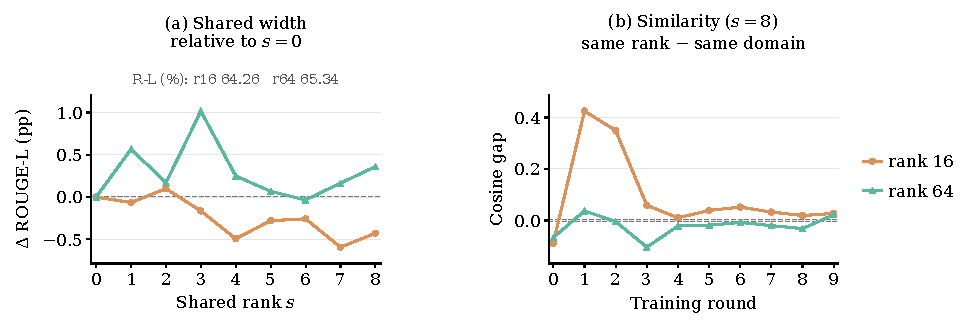
\includegraphics[width=0.8\linewidth]{figs/acl_motivation_flan_r16_64.pdf}
    \caption{Selective rank sharing on FLAN with eight clients and two rank budgets, 16 and 64 (four clients each), under Dirichlet $\alpha=0.5$.
    (a) Rank-group ROUGE-L changes as the shared-prefix width $s$ varies, relative to each group's matched $s=0$ run; the corresponding absolute ROUGE-L scores are shown above the panel.
    At $s=8$, ROUGE-L decreases for rank 16 and increases for rank 64.
    (b) In an independent $s=8$ run, we plot the mean cosine of effective shared-upload changes for same-rank/different-domain pairs minus that for same-domain/different-rank pairs over R0--R9.
    The two rank groups exhibit different alignment trajectories; diagnostic details are given in \appref{sec:appendix:motivation-setup}.}
    \label{fig:acl-motivation}
\end{figure}

\section{Related Work}
\label{sec:related}

\boyi{
\fakeparagraph{Federated LLM Fine-tuning}
Federated LLM fine-tuning collaboratively adapts a pretrained language model on decentralized private corpora without collecting raw client data.
FedIT explores federated instruction tuning~\cite{zhang2024fedit}, while FFA-LoRA improves the efficiency of LoRA-based federated adaptation~\cite{sun2024ffalora}.
Recent studies further personalize federated fine-tuning for non-IID clients: 
FedDPA combines global and local adapters at inference~\cite{yang2024feddpa}, FedLEASE allocates domain-specific LoRA experts by representation similarity~\cite{wang2025fedlease}, and FedTreeLoRA organizes layer-wise sharing through a client hierarchy~\cite{bian2026fedtreelora}.
These methods personalize adapter sharing or selection, but generally retain shape-compatible LoRA modules across clients and do not address resource-driven rank heterogeneity.
In contrast, we focus on resource-driven model heterogeneity, where clients fine-tune LoRA adapters with different ranks.
}

\boyi{\fakeparagraph{Federated LLM Fine-tuning with Rank Heterogeneity}}
A recent line of work lets the LoRA rank vary with client resources.
FLoRA stacks zero-padded adapters into a common wide matrix~\cite{wang2024flora}.
FlexLoRA aggregates full-size update matrices and redistributes rank by SVD truncation~\cite{bai2024flexlora}.
HETLoRA sparsely aggregates self-pruned updates of different ranks~\cite{cho2024hetlora}.
PF$^2$LoRA instead learns per-client ranks with a two-level sparsity regularizer~\cite{hao2025pf2lora}.

\boyi{
Nevertheless, these methods mainly determine how heterogeneous updates are aligned or decomposed at the server. 
Within each client's fixed rank budget, we study two coupled questions:
how much capacity to allocate to sharing, and which clients should influence its shared update and by how much.
The value of an allocation depends on the collaboration relationships, while the allocation shapes the updates available for collaboration.
}

\section{Problem Statement}
\label{sec:problem}

\subsection{Preliminaries}

\fakeparagraph{Federated LoRA Fine-tuning}
We consider federated fine-tuning across $n$ clients, where client $i$ keeps its dataset $\mathcal{D}_i$ private and adapts a frozen LLM backbone $\phi$ through a LoRA module.
Let $\omega_i=|\mathcal{D}_i|/\sum_{k=1}^{n}|\mathcal{D}_k|$ denote the fraction of training examples held by client $i$, with $\sum_{i=1}^{n}\omega_i=1$.
In the standard homogeneous-rank setting, all clients optimize a shared adapter with factors $B\in\mathbb{R}^{d_{\mathrm{out}}\times r}$ and $A\in\mathbb{R}^{r\times d_{\mathrm{in}}}$.
With the LoRA scaling absorbed into the factors and the layer index omitted, the federated objective is
\begin{equation}
    \min_{B,A}
    \sum_{i=1}^{n}\omega_i
    \mathcal{L}_i\!\left(\phi+BA;\mathcal{D}_i\right),
    \label{equ:objective}
\end{equation}
where $\mathcal{L}_i$ is the mean training loss on client $i$'s local dataset.
Clients optimize local copies of the common factors, which the server coordinates toward the shared adapter $BA$.


\fakeparagraph{Federated LoRA Fine-tuning with Rank Heterogeneity}
In resource-heterogeneous deployments, client $i$ may instead operate under a fixed, client-specific rank budget $r_i$~\cite{bai2024flexlora,wang2024flora,cho2024hetlora}.
Under these client-specific feasible sets, the learning target becomes
\begin{equation}
    \begin{aligned}
        \min_{\{B_i,A_i\}_{i=1}^{n}}\quad
        &\sum_{i=1}^{n}\omega_i
        \mathcal{L}_i\!\left(\phi+B_iA_i;\mathcal{D}_i\right) \\
        \text{s.t.}\quad
        &B_i\in\mathbb{R}^{d_{\mathrm{out}}\times r_i},\quad
        A_i\in\mathbb{R}^{r_i\times d_{\mathrm{in}}},\quad i=1,\ldots,n,\\
        &\left|\{r_i:i=1,\ldots,n\}\right|>1.
    \end{aligned}
    \label{equ:heterogeneous-objective}
\end{equation}
The final constraint makes rank heterogeneity explicit by requiring heterogeneous client budgets.
Although the effective updates $B_iA_i$ share the common shape $d_{\mathrm{out}}\times d_{\mathrm{in}}$, their factor matrices have incompatible inner dimensions and therefore cannot be directly averaged across different ranks.
Consequently, federated knowledge transfer across heterogeneous adapters must preserve each client's rank budget while accounting for its local adaptation needs.

\fakeparagraph{Solution: Selective Rank Sharing}
To enable cross-client knowledge transfer without changing client $i$'s fixed budget $r_i$, we use a globally shared prefix of width $s$ and a client-specific protected remainder of width $p_i=r_i-s$ (see \figref{fig:selective-rank-sharing}).
Using subscripts $s$ and $p$ for the corresponding factor blocks, we write
\begin{equation}
    B_iA_i=B_{i,s}A_{i,s}+B_{i,p}A_{i,p},
    \qquad p_i=r_i-s,\quad s\in\{0,\ldots,\min_{1\le k\le n}r_k\}.
    \label{equ:selective-partition}
\end{equation}
Both blocks remain trainable.
After local training, the server aggregates the shared blocks separately for $B$ and $A$ using the same sample-size weights:
\begin{equation}
    \bar{B}_{s}=\sum_{i=1}^{n}\omega_i B_{i,s},
    \qquad
    \bar{A}_{s}=\sum_{i=1}^{n}\omega_i A_{i,s},
    \qquad
    \sum_{i=1}^{n}\omega_i=1.
    \label{equ:selective-aggregation}
\end{equation}
The server broadcasts $(\bar{B}_{s},\bar{A}_{s})$ to synchronize the shared prefix, while each client retains its protected block locally.
Selective rank sharing therefore controls how much of each heterogeneous adapter receives common external knowledge while preserving each client's total rank budget.





\subsection{Research Challenges}
\label{sec:problem:challenges}

Selective rank sharing preserves each client's fixed budget while allowing cross-client knowledge transfer, but it raises two coupled research challenges.
\begin{itemize}
    \item \textbf{How should a global receiving width be selected under heterogeneous rank budgets?}
    With a globally shared width $s$, client $i$ retains protected capacity $p_i=r_i-s$ within its fixed budget $r_i$.
    \figref{fig:acl-motivation}(a) shows that performance fluctuates as the shared rank changes and that the rank-16 and rank-64 groups respond differently on FLAN.
    At $s=8$, rank-16 clients lose ROUGE-L relative to $s=0$, while rank-64 clients gain.
    Moreover, the same width occupies different fractions of their budgets.
    These variations motivate dynamically selecting the global width $s$ rather than fixing it in advance.

    \item \textbf{How should the influence of external updates be adapted under coupled data and structural heterogeneity?}
    Clients differ in both their local data and their adapter rank.
    \figref{fig:acl-motivation}(b) shows that the relative similarity associated with matching rank versus matching domain differs across rank groups and training rounds.
    The rank-16 cosine gap remains positive from R1 onward, whereas the rank-64 gap changes sign across rounds.
    Thus, the relationship between client updates reflects both structural and data heterogeneity.
    Naive averaging may overlook client-dependent differences among contributions, motivating a \textit{fine-grained collaboration} mechanism.
\end{itemize}

Moreover, the two challenges are \textit{coupled}, as illustrated in \figref{fig:compound-heterogeneity}.
\begin{itemize}
    \item The allocation mechanism determines the subspace in which external influence may enter.
    This constrains the external knowledge available to the collaboration mechanism.
    \item The collaboration mechanism determines how strongly external knowledge is applied, which in turn affects the utility of the selected global width.
\end{itemize}
We therefore seek to coordinate both allocation and collaboration, so each client can adaptively absorb useful external knowledge while preserving its fixed budget and local adaptation needs.

\begin{figure}[t]
    \centering
    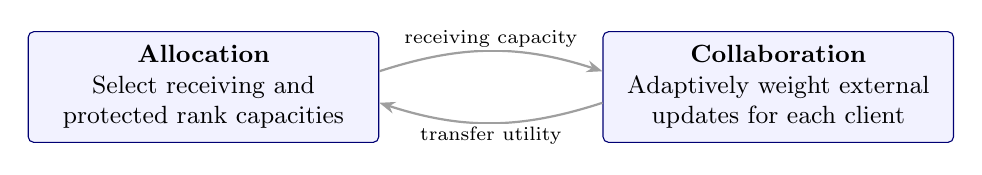
\begin{tikzpicture}[
        factor/.style={draw=blue!45!black, fill=blue!5, rounded corners=2pt,
            text width=4.1cm, minimum height=13mm, align=center, inner sep=5pt,
            font=\small},
        flow/.style={-{Stealth[length=2mm]}, thick, draw=gray!75}
    ]
        \node[factor] (allocation) at (0,0) {\textbf{Allocation}\\Select receiving and protected rank capacities};
        \node[factor] (collaboration) at (7.3,0) {\textbf{Collaboration}\\Adaptively weight external updates for each client};
        \draw[flow] ([yshift=2mm]allocation.east)
            to[bend left=18] node[midway, above, font=\scriptsize, fill=white, inner sep=1pt]
            {receiving capacity} ([yshift=2mm]collaboration.west);
        \draw[flow] ([yshift=-2mm]collaboration.west)
            to[bend left=18] node[midway, below, font=\scriptsize, fill=white, inner sep=1pt]
            {transfer utility} ([yshift=-2mm]allocation.east);
    \end{tikzpicture}
    \caption{Compound Impact of Allocation and Collaboration.}
    \label{fig:compound-heterogeneity}
\end{figure}
\FloatBarrier

\section{Method}
\label{sec:method}

% 2026-10-14: retain the complete-contribution and receiving-operator definitions from Section 39.
% Collaboration scoring, strength selection, and dependent allocation rules are pending redesign.
% Sources: ../FedLLM/ACL_Logs/method-39_progressive_recipient_allocation.md;
% ../FedLLM/exp/_archive_exps/1003_acl_progressive_exchange/design/progressive_allocation_report.md;
% ../FedLLM/alg/acl_1003_progressive_exchange.py and ../FedLLM/utils/progressive_{allocation_utils,metric}.py.
% Paper s_i denotes receiving capacity; the implementation calls it q_i.
% Writing references: ref/FedMosaic_SIGIR26_CR and ref/DarkDistill_KDD25_CR; see WRITING_STYLE.md.

\TODO{Section 4.1 Overview}

\TODO{Section 4.2 Allocation}
\TODO{Take collboaration weight into method design}

\TODO{Section 4.3 Adaptive Collaboration}
\TODO{Take allocation result into method design}

\TODO{Section 4.4 Putting it Together}

\subsection{Overview}
\label{sec:method:overview}

\fakeparagraph{Key Idea}
Under rank heterogeneity, a client should not have to choose between exposing its
entire adapter and receiving no external knowledge.
\sysname therefore decouples contribution from reception.
Each client contributes its complete locally trained adapter to a round-level pool,
while only a client-specific portion of its fixed rank budget is exposed to
incoming updates.
For client $i$, the receiving capacity $s_i$ and protected capacity $p_i=r_i-s_i$
determine where external knowledge may enter, whereas a client-specific
collaboration strength determines how much of that knowledge is applied.
This separation preserves the client's total rank budget and local adaptation
capacity while allowing useful cross-client transfer.

\fakeparagraph{Challenge-to-Component Map}
This design follows the two challenges in \secref{sec:problem:challenges}.
The allocation module determines how client $i$ divides its fixed budget $r_i$
between receiving and protected capacity, rather than imposing one sharing width
on all clients.
The collaboration module then determines whether the available external influence
benefits client $i$ and, if so, how strongly it should be applied.
The final putting-it-together procedure coordinates these decisions with complete
contribution, so restricting a client's reception does not remove its knowledge
from the pool available to other clients.

\fakeparagraph{Workflow}
At the beginning of each round, clients locally train both portions of their
adapters under the fixed budgets in \equref{equ:heterogeneous-objective} and
contribute their complete effective updates.
The server constructs the external target for client $i$ from the other clients'
updates using fixed training-size weights, as in \equref{equ:acl-target}.
The allocation module selects a receiving capacity $s_i$ and thereby protects
$p_i=r_i-s_i$ components.
Given this capacity, the collaboration module constructs the residual between
the external target and client $i$'s local update in the permitted subspace and
selects its reception strength, including zero when external influence is not
useful.
The final update is applied only to the receiving portion, producing the
personalized adapter used in the next round; the protected portion remains
untouched by direct incoming modification.

\fakeparagraph{Architecture}
\begin{itemize}
    \item \textbf{Allocation Module (\secref{sec:method:allocation}).}
    It determines the client-specific capacity $s_i$ within the fixed rank
    budget and reserves the remaining capacity for local adaptation.
    \item \textbf{Collaboration Module (\secref{sec:method:collaboration}).}
    It computes the external influence available within the selected receiving
    subspace and determines its client-specific reception strength.
    \item \textbf{Putting It Together.}
    It orders complete contribution, capacity allocation, and selective reception
    into one round-level procedure, while freezing the contribution pool before
    applying incoming updates.
\end{itemize}

Together, these components turn selective rank sharing into a coordinated
allocation-and-collaboration process: allocation controls where external
knowledge may enter, collaboration controls whether it should enter, and the
round procedure preserves complete contribution across clients.
The following subsections detail these components in the same order as the
workflow.

\subsection{Local Training and Complete Contribution}
\label{sec:method:contribution}

For the proposed client-specific allocation, client $i$ partitions its adapter as
\begin{equation}
    B_iA_i=B_{i,s}A_{i,s}+B_{i,p}A_{i,p},
    \qquad p_i=r_i-s_i,\quad s_i\in\{0,\ldots,r_i\}.
    \label{equ:capacity-partition}
\end{equation}
Client $i$ minimizes its local term in \equref{equ:heterogeneous-objective} from its preceding personalized state, training both portions in \equref{equ:capacity-partition} with total width $r_i$ and LoRA scaling fixed.
It then uploads the complete adapter, including the protected components, so that reducing its reception permission does not remove its knowledge from the contribution pool.
Within a round, $B_i,A_i$ denote the factors after local training, with scaling absorbed as in \secref{sec:problem}.
The server pools the other clients' complete effective updates into
\begin{equation}
    M_{-i}=\sum_{j\ne i}w_{ij}B_jA_j,
    \qquad
    w_{ij}=\frac{|\mathcal{D}_j|}{\sum_{k\ne i}|\mathcal{D}_k|},
    \label{equ:acl-target}
\end{equation}
where $|\mathcal{D}_j|$ counts local training examples, excluding selection data.
This forms an all-to-all contribution pool with every other client as an available source and training-size weights for the pooled target.
The donor proportions are fixed across candidate widths, leaving the receiving subspace and strength to determine how the pooled knowledge affects each client.
The server freezes all uploads before constructing receiving directions, so a change made during reception enters other clients' targets only in the next round.
Without an external contribution, the client retains its local state.

\subsection{Reception at a Given Capacity}
\label{sec:method:collaboration}

\fakeparagraph{Constructing the Receiving Direction}
For a candidate width $s$, we permit reception into the first $s$ native components and protect the remaining $r_i-s$ components.
Component identities retain their native order across rounds.
Since equal component indices need not represent the same directions across clients, we compare their complete effective updates and project the difference into client $i$'s permitted subspace.
For $s>0$, the server computes
\begin{equation}
    \Delta B_{i,s}=(M_{-i}-B_iA_i)A_{i,s}^{\dagger},
    \label{equ:acl-direction}
\end{equation}
where $A_{i,s}^{\dagger}$ is the Moore--Penrose pseudoinverse.
With strength $\lambda\in[0,1]$, reception gives
\begin{equation}
    \begin{aligned}
        B_i(s,\lambda)&=[\,B_{i,s}+\lambda\Delta B_{i,s},\ B_{i,p}\,],
        \qquad A_i(s,\lambda)=A_i,\\
        B_i(s,\lambda)A_i
        &=B_iA_i+\lambda(M_{-i}-B_iA_i)A_{i,s}^{\dagger}A_{i,s}.
    \end{aligned}
    \label{equ:acl-receive}
\end{equation}
The projection transfers the part of the residual represented in the selected row space, while changing only the receiving $B$ columns.
Subtracting the complete local update accounts for content already retained in the protected block; the direction vanishes when the complete local and external updates coincide.
The adapter retains $r_i$ component slots and algebraic rank at most $r_i$.
Zero width or zero strength preserves the original factors exactly.

\fakeparagraph{Collaboration Metric}
\TODO{Define a computable collaboration metric and its use in selecting reception strength, including zero reception, after the design and corresponding experiments are ready.}

\subsection{Progressive Capacity Allocation}
\label{sec:method:allocation}

\TODO{Reformulate capacity comparisons and update rules around the new collaboration metric once it is defined and evaluated.}

\section{Experiments}
\label{sec:exp}

The FLAN motivation studies in \figref{fig:acl-motivation} examine a fixed shared-prefix protocol with eight clients and ranks 16 and 64.
We report available federated LoRA baselines on NI and GLUE for context.
\TODO{Add the method comparison after the collaboration metric is defined and the corresponding experiments are complete.}

\subsection{Datasets}
\label{sec:exp:datasets}
We use the NI and GLUE Dirichlet $\alpha=0.5$ partitions, each with 16 clients.
The total rank budgets are 16, 32, and 64 for six, five, and five clients, respectively.
Each client has 200 test examples; the training and validation allocations for the reported methods are specified below.

\subsection{Evaluation}
\label{sec:exp:eval}
We report client-macro ROUGE-L (R-L) for Super-NaturalInstructions (NI) and GLUE.
For both datasets, each client generates answers on its test set, and the resulting client scores are averaged equally.
GLUE follows the project's causal generation protocol, so its reported metric is ROUGE-L rather than task-specific classification accuracy.

\subsection{Training Setup}
\label{sec:exp:environments}
The runs use Qwen3.5-0.8B and seed 615, with 10 main local optimizer steps per round and an effective batch size of eight.
We evaluate checkpoint R9 after ten communication rounds.
Method-specific optimizer phases and inference procedures incur additional computation beyond these main training steps.

\subsection{Main Results}
\label{sec:exp:results}
\tabref{tab:exp-ni-dir05} reports the available NI baselines.
\tabref{tab:exp-glue-dir05} reports the available GLUE baselines.

\begin{table}[t]
\centering
\small
\setlength{\tabcolsep}{4pt}
\caption{Client-macro ROUGE-L (\%) on Super-NaturalInstructions under Dirichlet $\alpha=0.5$.
The highest and second-highest scores are shown in bold and underlined, respectively.}
\label{tab:exp-ni-dir05}
\begin{tabular}{lr}
\toprule
\textbf{Method} & \textbf{ROUGE-L (\%)} \\
\midrule
LocalOnly                          & \textbf{57.5208} \\
FlexLoRA                           & \underline{54.7099} \\
FLoRA                              & 51.0599 \\
HetLoRA                            & 51.8617 \\
PF$^2$LoRA                          & 48.4953 \\
pFedLoRA                           & 51.3480 \\
FedRoRA                            & 53.6302 \\
Het-CPFLoRA                        & 54.0703 \\
\bottomrule
\end{tabular}
\end{table}

\begin{table}[t]
\centering
\small
\setlength{\tabcolsep}{4pt}
\caption{Client-macro baseline ROUGE-L (\%) on GLUE under Dirichlet $\alpha=0.5$.
The highest and second-highest scores are shown in bold and underlined, respectively.}
\label{tab:exp-glue-dir05}
\begin{tabular}{lr}
\toprule
\textbf{Method} & \textbf{ROUGE-L (\%)} \\
\midrule
LocalOnly                          & \textbf{79.9531} \\
FlexLoRA                           & \underline{79.9010} \\
FLoRA                              & 77.5885 \\
FedRoRA                            & 77.1719 \\
\bottomrule
\end{tabular}
\end{table}

\fakeparagraph{Comparison Scope}
PF$^2$LoRA uses shared rank 4 and private rank 12, 28, or 60 to match each client's total rank budget.
Het-CPFLoRA uses shared rank 12, 24, or 48 and its paper dynamic weighted inference protocol.
For NI, LocalOnly, FlexLoRA, FLoRA, and FedRoRA train on 936 examples per client with 64 held out, whereas HetLoRA, PF$^2$LoRA, pFedLoRA, and Het-CPFLoRA use all 1000 training examples.
The results therefore retain method-specific training-data and computation budgets.

\fakeparagraph{Observed Results}
Among the reported baselines, LocalOnly has the highest ROUGE-L on NI and GLUE.


\section{Conclusion}
\label{sec:conclusion}

We study how receiving capacity and external influence should be coordinated in federated LoRA with fixed heterogeneous rank budgets.
The motivation studies show uneven responses to a common sharing rule and varied update geometry, motivating client-specific assessment of collaboration.
\TODO{Complete the method and result summary after the collaboration metric and its experimental evidence are ready.}

\clearpage
%
% ---- Bibliography ----
%
% BibTeX users should specify bibliography style 'splncs04'.
% References will then be sorted and formatted in the correct style.
%
\bibliographystyle{splncs04}
\bibliography{refs}
%

\newpage
\appendix

\section{Motivation Study Setup}
\label{sec:appendix:motivation-setup}

% Sources: ../FedLLM/exp/_archive_exps/1023_flan1_motivation/PROTOCOL.md and
% ../FedLLM/exp/_archive_exps/1023_flan1_motivation/recovery_tail_01/report/flan8c/RESULTS.md.
% Frozen configurations: ../FedLLM/exp/_archive_exps/1023_flan1_motivation/configs/
% flan1_8c_two_ranks_dir05_q8.yaml and flan1_8c_two_ranks_dir05_geometry_q8.yaml.

This appendix details the shared-width study and the training-only similarity diagnostic in \figref{fig:acl-motivation}.

\fakeparagraph{Dataset and Clients}
The studies use eight task categories from FLAN~\cite{wei2022finetuned}: coreference, entailment, linguistic acceptability, paraphrase, question classification, structure-to-text generation, text formatting, and word disambiguation.
We use a Dirichlet $\alpha=0.5$ allocation across eight clients, balanced to give each client 300 training examples and 200 test examples with matching local train/test task proportions.
Four clients have fixed total rank 16, and the other four have rank 64.
The dataset and client rank assignments are shared by both studies and remain fixed across the width sweep.

\fakeparagraph{Model and Training}
Both studies use Qwen3.5-0.8B, seed 615, full client participation, and 10 communication rounds with 10 local optimizer steps per round.
The microbatch size is 2 with gradient accumulation over 4 microbatches, and the initial learning rate is $10^{-4}$, decayed by a factor of 0.99 per round.
The physical LoRA rank and scaling parameter are both 64, with active capacity fixed to each client's assigned rank and dropout 0.05.
The maximum sequence length is 2,048 tokens, reserving up to 512 tokens for the answer.
We use the base shared-prefix method: for shared width $s>0$, the $B$ columns and $A$ rows of the first $s$ LoRA components are averaged separately across all clients, including the receiving client, after each round, while the remaining active components stay local.
Aggregation is weighted by training sample count, giving equal weights here because all clients have 300 training examples.
Both portions participate in training and prediction; $s=0$ uses the same local training protocol with no shared components.
The same factor-averaging rule is used at every nonzero width, with no partner selection or fitted reception strength.

\fakeparagraph{Shared-Width Study}
For \figref{fig:acl-motivation}(a), all clients use a common shared width $s$, swept over $s\in\{0,\ldots,8\}$ while keeping the model, data, client ranks, seed, and training budget fixed.
We evaluate the final post-aggregation models at R9 on all 200 test examples per client and average ROUGE-L first within each client, then equally across the four clients in each rank group.
The plotted change is each group's mean at $s$ minus its own mean at $s=0$, in percentage points, using the full-precision saved client scores.
The rank-16 and rank-64 groups have $s=0$ ROUGE-L scores of $64.2584\%$ and $65.3399\%$, respectively.
The overall client means at $s=0$ and $s=8$ are $64.7991\%$ and $64.7644\%$, respectively.
The two rank groups contribute equally to the overall mean because each contains four clients.

\fakeparagraph{Similarity Diagnostic}
For \figref{fig:acl-motivation}(b), all clients use a fixed shared width $s=8$ in a separate training-only rerun, with a snapshot after every round and no test evaluation.
Its scientific configuration matches the corresponding width-sweep arm except for saving all round snapshots instead of only the final one.
R0 is the first completed training round, and R9 is the tenth and final round.
The diagnostic is computed separately for the total-rank groups 16 and 64.
Cosines compare the effective shared uploads $B_{\mathrm{upload}}A_{\mathrm{upload}}-B_{\mathrm{global}}A_{\mathrm{global}}$ relative to the pre-round global state, concatenated across all LoRA layers.
For each total rank $r$, the same-rank mean uses different-domain pairs with both clients at $r$; the same-domain mean uses same-domain pairs with different ranks and one client at $r$.
Domain denotes the recorded dominant task category.
Each rank group has six same-rank/different-domain pairs and one same-domain/different-rank pair, with membership fixed across rounds.
The same-domain reference is a single cross-rank pair with entailment as its dominant category, and both curves use this reference.
All selected cosines are defined in every round; the complete diagnostic contains 28 unordered pairs per round and 280 pair/round records in total.
Each curve plots the same-rank pair mean minus the same-domain pair mean, so positive values indicate higher same-rank cosine.

\fakeparagraph{Interpretation}
Both studies use one seed and provide no across-seed uncertainty estimate.
Rank groups differ in task composition, so their contrasts are descriptive rather than causal rank effects.
The matched $s=0$ arm permits within-protocol comparisons, but the test curves are descriptive and are not used to select shared widths.
Changing $s$ jointly changes protected capacity, exchanged content, and training, so these comparisons do not isolate donor-specific transfer or establish a general advantage for sharing.
The shared same-domain reference is sparse, and the two similarity curves are not independent repeats.
The two panels use separate runs and endpoints; the cosine diagnostic does not measure benefit to the target client or validate a partner-selection rule.
Because the averaging rule is fixed in the shared-width sweep, the two panels do not measure an allocation-by-collaboration interaction.

\fakeparagraph{Relation to the Proposed Method}
The probe couples reception and contribution through the same global width $s$ and averages the shared factors directly, following the selective rank sharing definition in \secref{sec:problem}.
In \secref{sec:method}, clients instead contribute their complete adapters, while $s_i$ limits the receiving subspace for a projected effective update.
Consequently, the probe supplies observations for the research questions, while evaluating the proposed reception rule requires its own matched controls.

\section{MMLU-Pro Baseline Results}
\label{sec:appendix:mmlu-baselines}

% MMLU-Pro is kept here pending the user's decision on its inclusion in the final paper.
\tabref{tab:exp-mmlu-dir05} reports client-macro multiple-choice (MC) accuracy on MMLU-Pro under Dirichlet $\alpha=0.5$.
The experiments use Qwen3.5-0.8B, seed 615, and the final checkpoint after 10 communication rounds.
The 13 clients have total rank budgets 16, 32, and 64, assigned to five, five, and three clients, respectively.
Accuracy is computed on each client's full original test set and averaged equally across clients.

\begin{table}[t]
\centering
\small
\setlength{\tabcolsep}{4pt}
\caption{Client-macro baseline MC accuracy (\%) on MMLU-Pro under Dirichlet $\alpha=0.5$.
The highest and second-highest scores are shown in bold and underlined, respectively.}
\label{tab:exp-mmlu-dir05}
\begin{tabular}{lr}
\toprule
\textbf{Method} & \textbf{MC accuracy (\%)} \\
\midrule
LocalOnly                          & 30.0322 \\
FlexLoRA                           & \textbf{31.9374} \\
FLoRA                              & \underline{30.5800} \\
\bottomrule
\end{tabular}
\end{table}

FlexLoRA has the highest MC accuracy among the reported baselines.


\end{document}
